\chapter{Multi-view Fusion Module and Fusion Network}
In this chapter, we introduce our learning-based framework, that is fully constitutional, for bottom-up 3D human pose estimation. 
\section{Backbone Module: ResNets}
Our backbone is the fully convolution network (FCN) based on ResNet50 that pretrain on COCO for the task of segmentation \cite{resnet50}. Similar to \cite{xiao2018simple}, we use the last stage of the convolutional layer $\bm{C4}$ of the pretrained model and a deconvolution head $\bm{D}$, shown in Fig. \ref{fig:2d-backbone} and Table \ref{tbl:2d-backbone}, to increase the resolution and reduce the number of channels form pretrained model. For each convolutional operation, a ReLU and a batch normalization operator are followed.

During training, we used Adam optimizer and train on COCO dataset. We fixed the pretrained model, except $\bm{C4}$. $\bm{C4}$ and $\bm{D}$ are trained together but with different learning rate with 0.0001 and 0.01. The smaller learning rate for $\bm{C4}$ is given because we only want to fine tune this layer for the 2D joint heatmap regression task. In addition, we do not crop and feed the network with regions with person bounding boxes, like many other 2D backbone being used in many other works. However, joints usually occupy a relative small areas in the images and overwhelm with negative examples, such as background. To effectively train our 2D backbone, we feed the down-sampled images from COCO and calculated a weighted loss with high penalty rate on places with joints. Recall (\ref{eq:joint-heatmap}) and the weighted L2 Loss $\mathit{L}$ is calculated as 
\begin{gather}
\mathit{L} = \sum_{k=1}^J\norm{\mathbf{W}_k \odot \left(\mathbf{H}_k - \mathbf{H}_{k_{GT}}\right)}^2
\label{eq:joint-heatmap}
\end{gather}
where
\begin{gather}
\mathbf{W}_k(\mathbf{x}) = 
\begin{cases}
	10,\ \text{if} & \mathbf{H}_{k_{GT}}(\mathbf{x})\geq \lambda \\ 
	1,& \text{otherwise}\\
\end{cases}
\end{gather}
We set $\lambda$ to 0.5 empirically, since we observe better quality in prediction.¸


\begin{table}[htpb]
	\centering
	\begin{tabular}{|c|c|c|c|c|c|c|}
		\toprule
		layer index & trans. conv2d & conv2d.\\
		\midrule
		1 & 2048, 1024, (4, 4), (2, 2), (0, 0) & 1024, 512, (3, 3), (1, 1), (0, 0)\\ \hline
		2 & 512, 256, (4, 4), (2, 2), (0, 0) & 256, 128, (3, 3), (1, 1), (0,0) \\ \hline
		3 & - & 128, 64, (3, 3), (1, 1), (1, 1) \\ \hline
		4 & - & 64, 55, (3, 3), (1, 1), (1, 1)\\ \hline
		\bottomrule
	\end{tabular}
\caption[Structure of deconvolution head]{Structure of deconvolution head. We list out the parameters of 2d convolutional operation in the following order: input channels, output channel, kernel size, stride, and padding}\label{tbl:2d-backbone}
\end{table}

\begin{figure}´
	\centering
	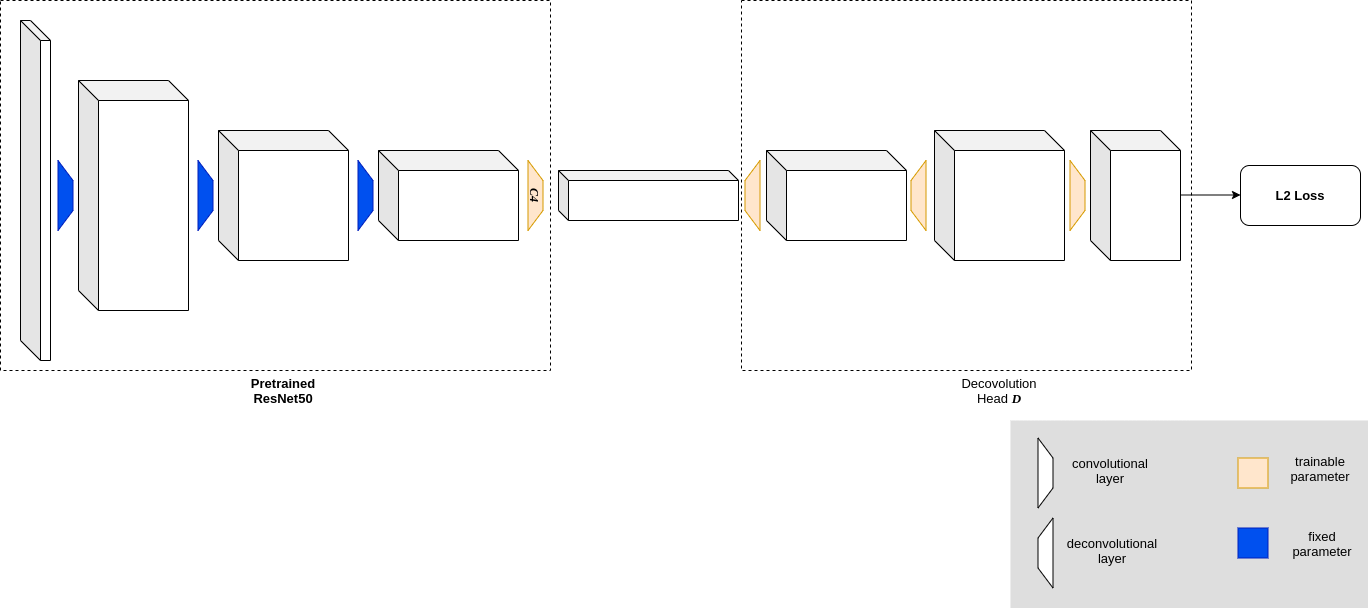
\includegraphics[width=1.0\columnwidth, height=0.5\columnwidth]{figures/ch5/2d-backbone-architecture.png}
	\caption{Overview of our 2D backbone. We train the last convolutional layer of the pretrained ResNet50 with the deconvolutional head together.} 
	\label{fig:2d-backbone}
\end{figure}


\section{Sampler Module: Epipolar Sampler}\label{ch4:fusion-module}
A 2D joint represented by heatmap $\mathbf{H}_k^{(v)}(\mathbf{x}^{(v)})$ from view $\mathit{v}$ might be occluded or has a low score due to lack of training examples (e.g. novel view angle). Is there a way to retrieve the heatmap score $\mathbf{H}_k^{(v')}(\mathbf{x}^{(v')})$ at the corresponding point $\mathbf{x}^{(v')}$ in other view $\mathit{v}'$, which the joint is has a higher score? According to (\ref{eq:epipolar-line}), we can estimate a point-to-line relationship for a pair of views if we know the extrinsic and intrinsic matrices of both views. If we sample enough points along the epipolar line on the joint heatmap $\mathbf{H}_k^{(v')}$, the sampled point with the highest score can the corresponding joint in another view, demonstrating Fig. \ref{fig:epipolar-sampler} (a) and (b).

The epipolar sampler $\mathit{E}$ outputs the maximum scores on the corresponding epipolar line of the joint heatmap. To explain in detail, given a heatmap score $\mathbf{H}_k^{(ref)}(\mathbf{x}^{(ref)})$ at pixel location $\mathbf{x}^{ref}$, where superscript $ref$ means at \textit{reference view} and subscript $k$ means $k$-th joint index, and the projection matrices, $\mathbf{P}_{src}$ and $\mathbf{P}_{ref}$, of source and reference view. We can sample a set of $N$ points $S^{(src)} = \left\{\mathbf{x}_{1}^{src}, \dots, \mathbf{x}_{N}^{src}  \right\}$ on the corresponding epipoloar line $\mathbf{l}$ at $\mathbf{H}_k^{(src)}$ from source view. We compare $N$ scores $\mathbf{H}_k^{(src)}(S^{(src)}) = \left\{\mathbf{H}_k^{(src)}(\mathbf{x}_{1}^{src}), \dots, \mathbf{H}_k^{(src)}(\mathbf{x}_{N}^{src}) \right\}$ on the epipolar line and retrieve the biggest one, see Fig. \ref{fig:epipolar-sampler} (b). Specifically,

\begin{gather}
	\mathit{E}(\mathbf{x}_{ref},\mathbf{P}_{ref}, \mathbf{P}_{src}) = 
	\max\left(
		\left\{\mathbf{H}_k^{(src)}(\mathbf{x}_{1}^{src}), \dots, \mathbf{H}_k^{(src)}(\mathbf{x}_{N}^{src}) \right\}
	\right)
\end{gather}

We can use $\mathit{E}$ for every pixel on the reference view and create a heatmap $\mathbf{H}_{ep}(\mathbf{x}_{ref})$ in the image space of reference view but contains the information from source view, shown in Fig. \ref{fig:epipolar-sampler} (c). Moreover, we can integrate more source views rather than just one, shown in Fig. \ref{fig:epipolar-sampler} (d).

\begin{figure}
	\centering
	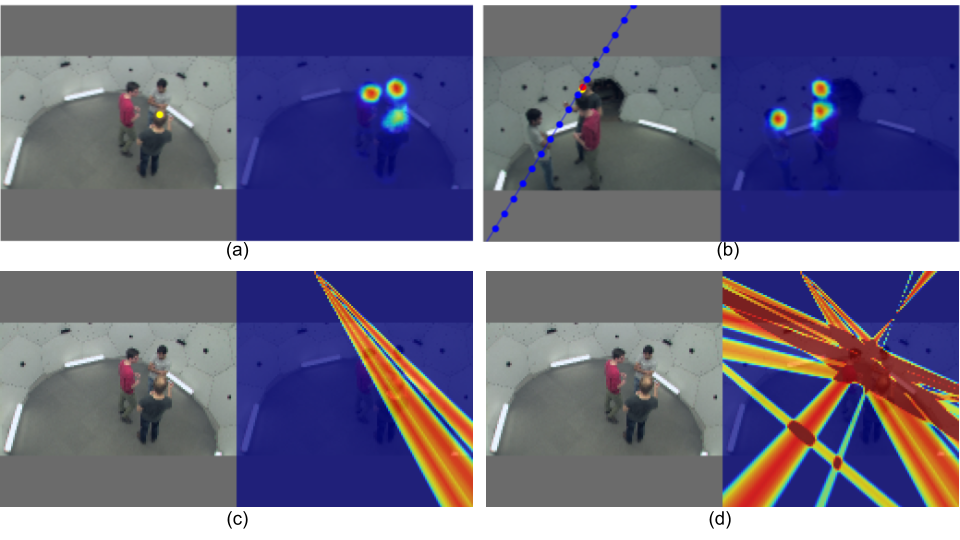
\includegraphics[width=1.0\columnwidth]{figures/ch4/epipolar-sampler.png}
	\caption{Illustration of Epipolar Sampler $\mathit{E}$. Image from a view is on the left and the joint heatmap is on the right side. Only nose joint is visualize (a) An occluded nose joint (yellow circle) has low score in view $\mathit{v}$ (b) The corresponding epipolar line in the other view $\mathit{v}'$. The same nose joint (yellow circle) is near the maximum (red circle) of all sampled points (blue circle) on the epipolar line (c) retrieved maximum for every point on view $\mathit{v}$ (d) Output of Epipolar Sampler $\mathit{E}$, by integrate 4 different views.} 
	\label{fig:epipolar-sampler}
\end{figure}
\section{View Fusion}
The architecture of view fusion network is based on UNet. For comparison of the view fusion network, we create (1) a baseline model, where the convolution layer is compose by 3D convolutional kernels and the input are heatmaps from multiple views (2) a fusion network, where the convolutional layer is compose by 2D convolutional kernels and the input is a heatmap $\mathbf{H}_{ep}$ gernerated by epipolar sampler $\mathit{E}$ . 
\subsection{Baseline Model}
In the baseline model, the input of the model is 3D heatmaps from 5 different views and the predict heatmaps for these 5 views. The convolutional kernels are 3D, where the first two dimension are 3-by-3 but the third dimension is fully connect with the heatmaps from 5 different views. We would like to compare the model with the view fusion network that has use the output of epipolar sampler $\mathbf{H}_{ep}$, shown in Fig. \ref{fig:epipolar-sampler} (d), which aggregates multi-view information within a single view. The model has UNet-like overall architecture, but a ResNet-like convolutional block.
\begin{figure}
	\centering
	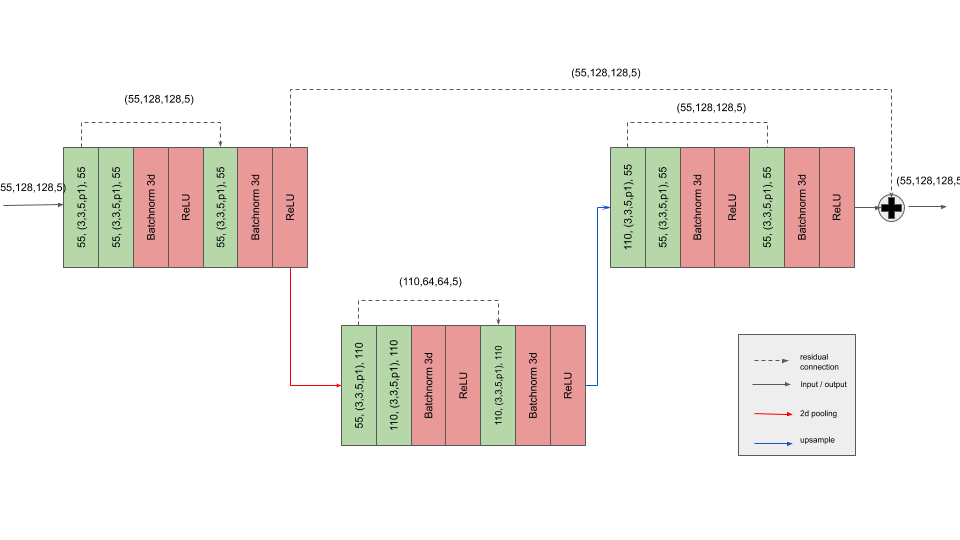
\includegraphics[width=1.0\columnwidth]{figures/ch4/baseline.png}
	\caption{Overview of the baseline model, where the green blocks are 3d convolutional kernels with input channel, (width, height, depth, 2d padding), and output channel. Instead of concatenating, we use residual connections to reduce number of parameters. We also show tensor sizes in parentheses for a sample of input and prediction, where (55, 64, 64, 5) denotes 55 channels, 64 width, 64 height, and 5 different camera views.}
	\label{fig:view-baseline}
\end{figure}
\subsection{View Fusion Model}
The view fusion model takes heatmap $\mathbf{H}_{ep}$ and concatenating with heatmap $\mathbf{H}^{ref}$ from reference view, thus the number of channels at the input is 110 (channels from reference view 55 plus 55 channels from epipolar sampler). In additon, the number of parameters between baseline and fusion model is the same. Although fusion model has more layer, it only use 2d convolution kernels. 
\begin{figure}
	\centering
	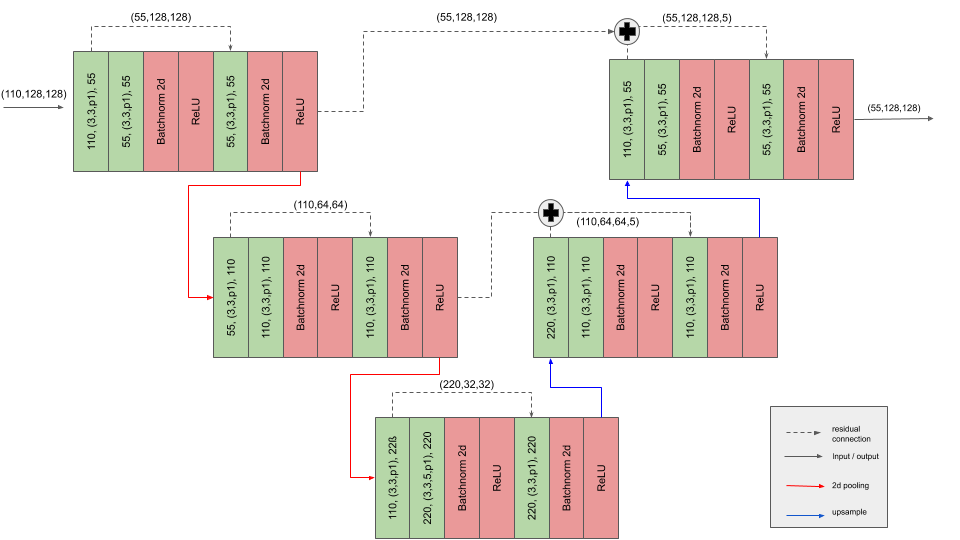
\includegraphics[width=1.0\columnwidth]{figures/ch4/view-fusion.png}
	\caption{Overview of the fusion model, where the green blocks are 2d convolutional kernels. The  with input channel, (width, height, 2d padding), and output channel.}
	\label{fig:view-baseline}
\end{figure}

\section{Temporal Fusion Model}
In temporal fusion model, we use 3d convolutional kernels like baseline model but the third dimension operates on time domain. The time resolution decrease because we do not use padding at time domain during convolution operation in the contractive path. In the expansive path, we feed the output of contractive path to the input of convolution layer, since the contractive path has higher definition in time domain.
\section{Summary}
Our full framework is composed of 3 models: a 2D joint estimation backbone, an epiploar sampler, a fusion model and a temporal fusion model. All the source views are merge at the epipolar sampler and refine at the view fusion model. Then, all the frames are merge into one at the temporal fusion model. The framework, shown in Fig. \ref{fig:full-framework} capture both time and spatial information from multi-view video.
\begin{figure}
	\centering
	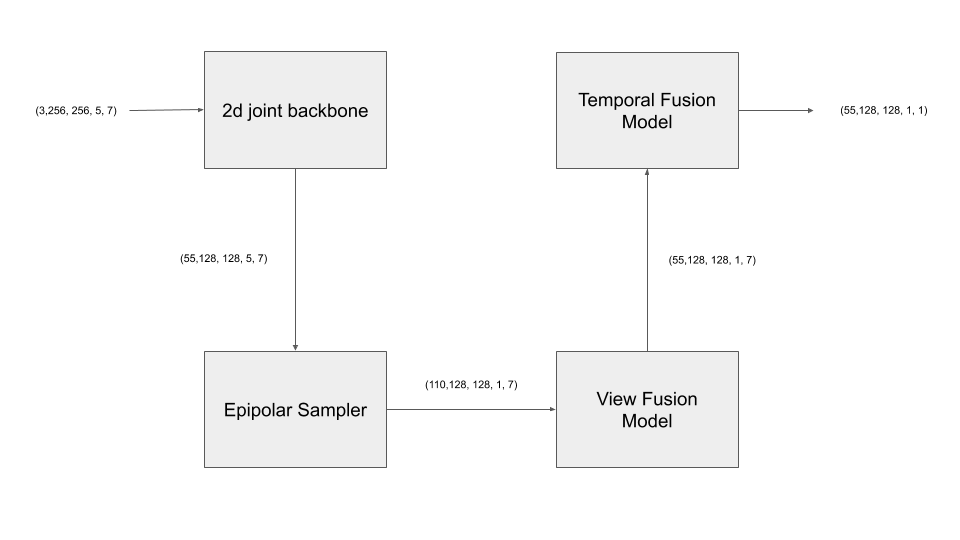
\includegraphics[width=0.7\columnwidth]{figures/ch4/full-model.png}
	\caption{Our complete framework covers both time and spatial domain. The parenthesis describe the dimension of input and output tensor, it means (channels, height, width, camera view, number of frame).}
	\label{fig:full-framework}
\end{figure}
\begin{figure}
	\centering
	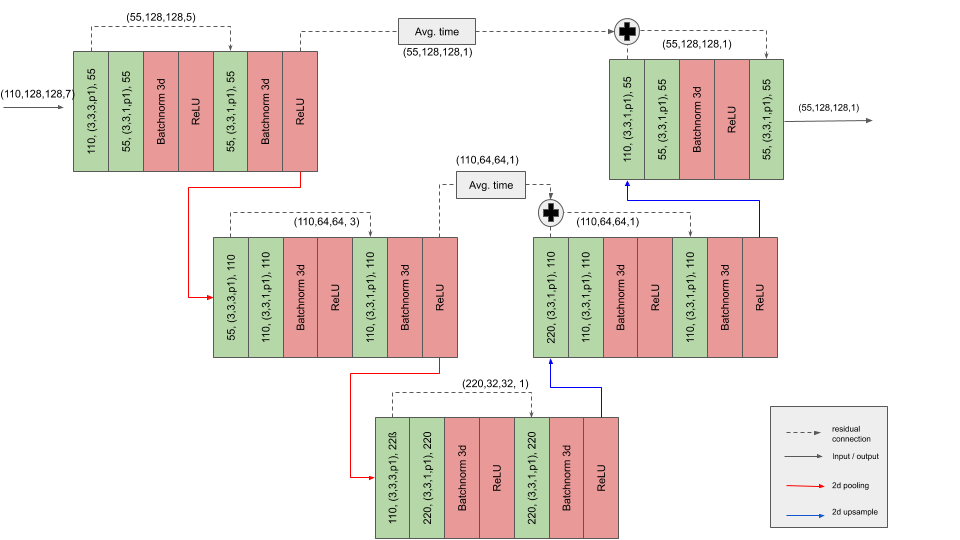
\includegraphics[width=1.0\columnwidth]{figures/ch4/temporal-fusion.png}
	\caption{Overview of the fusion model, where the green blocks are 2d convolutional kernels with input channel, (width, height, depth, 2d padding), and output channel.}
	\label{fig:view-baseline}
\end{figure}
\begin{figure}
	\centering
	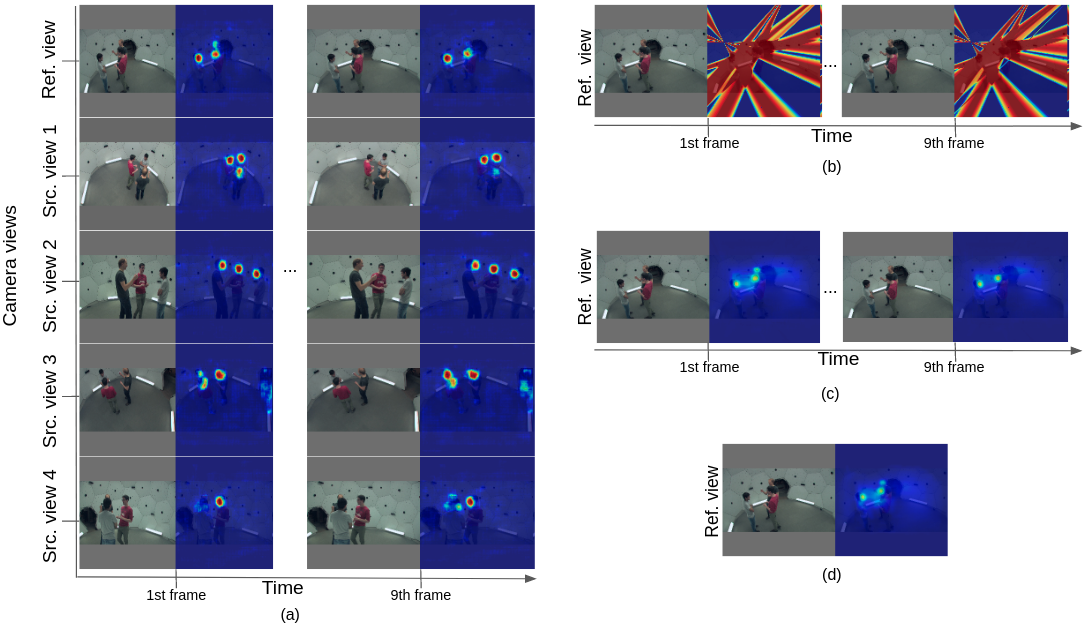
\includegraphics[width=1.0\columnwidth]{figures/ch4/full-framework-heatmap.png}
	\caption{Predicted sample from the start (a) to the end (e) of our framework. (a) The output of 2D joint backbone at different frame and across 5 different views, one reference view and 4 other source views. (b) The output of epipolar sampler. All the pixels on reference view sample from 4 different source views using epipolar geometry. (c) The output of fusion net that takes the epipolar heatmap at (b) as input. (d) The output of temporal fusion net that merge multiple frames into one.}
	\label{fig:full-framework-heatmap}
\end{figure}